% vim:ft=tex

\section{Prediction on Hourly Basis}

\subsection{Data Preparation}

% Sliding windows, ...
% Aggregation stuff...

\subsubsection{Holidays}

To add the bank holidays are day-based, so they should be set on a 24 hour windows.
However, fixing the bank holidays from midnight to midnight the next day might not
be the best solution as people might consider the evening of a bank holiday the same
way as they do for normal week day, while the evening of the day before will be more
interesting. Indeed, when people want to go out in the evening and go to bed late,
they will prefer doing that when they don't have to wake up early in the morning,
thus they may be more likely to use a bike the end of the day before the bank
holiday than of the day itself.

This is why it might be a good idea to test the accuracy of the prediction
placing bank holidays from 6pm the day before to 6pm the day itself.

% TODO: accuracies
% The accuracy of the overall model on the testing data using the bank-holidays
% starting at 6pm is []. When not using this, we get a lower accuracy of
% [].
% TODO: RMSE ?

\subsection{Learning and Prediction}

For the learning part, we used the same algorithm as described in~\ref{data_prediction}.
We trained twenty-four models, one per future hour to predict.
For each model, we only use the past and current data which we match to
the future expected number of rented bike for the given following hour,
no other future data is used.

We used the sliding-windows hourly based data over 48 hours (aggregating per slice
of 6 hours after the first 24 hours).
We have an accuracy of 0.800638 on the test dataset.
On the graph below, you can see several randomly selected days in the testing set
starting at midnight and predicting for the whole day. The title above each graph
indicates the date displayed, the actual expected value is in red and the
predicted one is in blue.
\begin{figure}[H]
\hspace{-0.9cm}
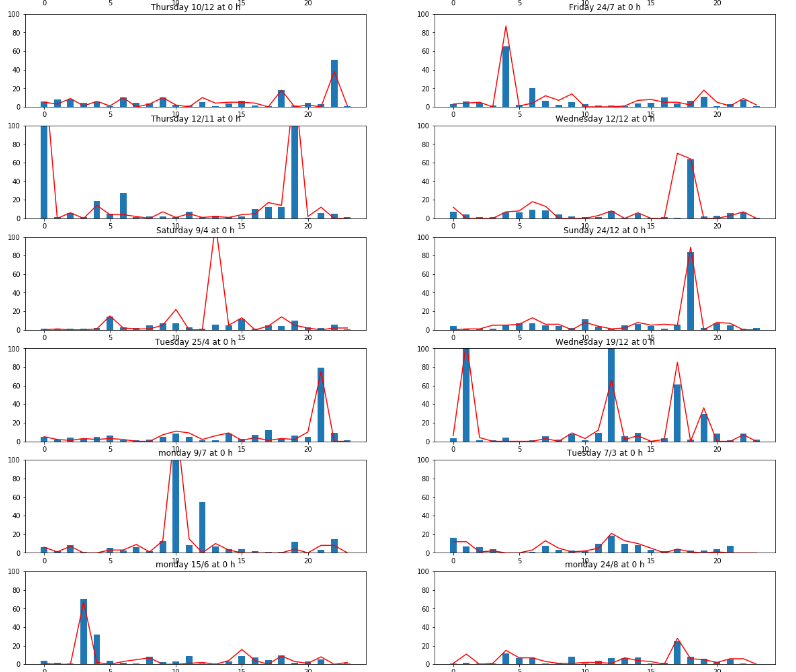
\includegraphics[width=1.1\textwidth]{img/hourly_predictions}
\captionof{figure}{Comparison of expected (red) and predicted (blue) hourly rented bikes on test dataset}\label{fig:hourly_pred}
\end{figure}

As we can see on the Figure~\ref{fig:hourly_pred} and considering the measured accuracy,
we can see that we can predict quite well the amount of rented bikes for the following
24 hours based on the data of the previous 48 hours.
